\documentclass[11pt]{article} %{{{

\usepackage{amsmath}
\usepackage{amssymb}
\usepackage{graphicx}
\usepackage{url}
\usepackage[usenames,dvipsnames,svgnames,table]{xcolor}
\definecolor{light-gray}{gray}{0.8}
\def \del #1{ {\color{light-gray}{#1}} }
\def\yy#1{\footnote{\color{red}\textbf{#1 -YY}} }
\def\ej#1{\footnote{\color{blue}\textbf{#1 -EJ}} }
\usepackage{hyperref}


\usepackage[backend=bibtex]{biblatex}
\addbibresource{main.bib}
\graphicspath{ {./figs} }

\usepackage{array}
\usepackage{subcaption}
%}}}

\begin{document} %{{{

\title{Evolution of Fanfictions in Fandoms} %{{{
\date{\today}
\maketitle %}}}

\section{Introduction} %{{{
\label{sec:introduction}
\paragraph{} Many creative cultural products in human history are centered around a common topic and developed into different versions through time and interaction between creators. Myths and folktales in oral traditions of civilizations around the world often follow this pattern, for example, the tale of the Little Red Riding Hood or Mahabharata. 

In the contemporary pop culture, this tradition is sometimes found in a new form --- fanfictions. 

\paragraph{}Transformative works, or in a more common term, fan works, are one typical kind of production from fandoms\cite{wiki:transf_work}. These are creative works made by fans based on one or more original works, and are often centered around certain characters or story lines. For example, a story written by a contemporary fan about Sherlock Holmes in his retirement is considered a fan fiction in the Sherlock Holmes fandom. Although fan works contain multiple media types such as art, music and games, one of the most common type is creative writing--fanfictions.

\paragraph{} This project studies the evolution of fanfictions in fandoms. Data for the study comes from Archive of Our Own (AO3). This site hosts fan works --- mainly fanfictions --- that users upload and their metadata, and categorizes them based on fandoms. Established in 2010, it has become one of the most popular transformative work archives. We collected fanfictions from 42 fandoms according to AO3's list of most popular fandoms as of March 2016 \footnote{from this list: \url{http://archiveofourown.org/media}}. \ej{The page lists 50 fandoms, 5 for each category; there are some overlappings, after removing which 42 are left. Still some of these can have heavy overlappings (eg. ``Marvel" and ``Marvel movies". I might remove these as well.}
We only kept the fictions written in English, which leaves us with 3,726,307 fictions. The number of fictions in each fandom is shown in Figure \ref{fig:fandom_size}.

\begin{figure}[htbp]
\begin{center}
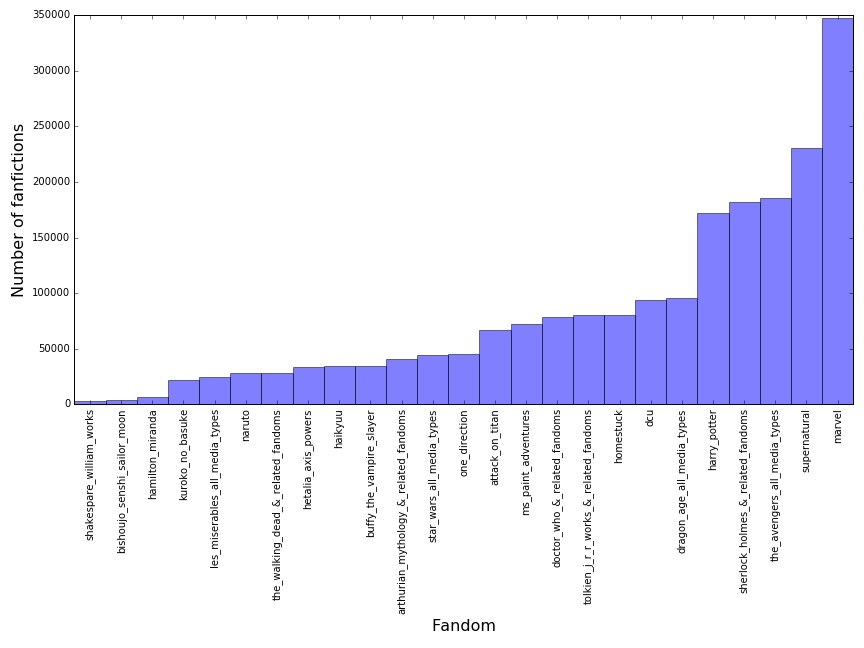
\includegraphics[width=0.9\textwidth]{/fandom_size.png}
\caption{Number of fanfictions in each fandom}
\label{fig:fandom_size}
\end{center}
\end{figure}


\paragraph{} Besides the work texts, we also collected metadata including 23 fields that can be roughly divided into two categories. One is tags generated by the author, which describes the works' contents; the other is tags that are automatically generated, and describes the works’ other information, as well as the readers' feedback. Table \ref{tab:metadata} gives the names of these fields. 

\begin{table}[htp]
\caption{Metadata of the writings}
\begin{center}
\begin{tabular}{p{3cm}|p{3cm}|p{3cm}|p{3cm}}
  \hline			
 \multicolumn{2}{c}{ Content related} & \multicolumn{2}{c}{Non-content related}\\ 
 User-generated & Not-user-generated &  User-generated & Not-user-generated \\
\hline
Additional Tags, Characters, Relationship, Summary, Text, Title
 & Fandoms,  Archive Warnings, Category, Rating
&  Notes
& Author, Bookmarks, Chapter Index, Chapters, Comments, Complete Date, Hits, Kudos, Language, Publish Date, Update Date, Word Count\\
\hline
\end{tabular}
\end{center}
\label{tab:metadata}
\end{table}%

\paragraph{} Among the metadata fields, we're especially interested in the fields ``Hits" and ``Kudos", which shows how many times a fiction has been clicked or liked by readers. These are useful proxies for the popularity of a piece of work in a specific fandom.

\paragraph{} We model the fictions with a unigram language model. The Good-Turing smoothing\cite{gales1995good} is applied to assign non-zero probabilities to previously unseen unigrams. When creating the unigram list, we also remove the rare unigrams that appear in less than 5 documents.

\begin{figure}[htbp]
\begin{center}
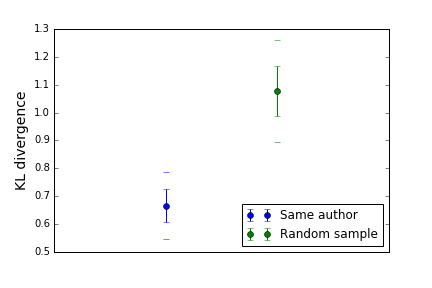
\includegraphics[width=0.6\textwidth]{/kl_validation.png}
\caption{KL divergence between fictions from the same author and fictions from different authors in the Shakespeare fandom. The blue point: the author with highest number of fictions in this fandom. The average KL divergence between each pair of his/her fictions is computed with error bar generated by bootstrap resampling. The green point: The computation repeated on a random example with the same size.}
\label{fig:kl_validation}
\end{center}
\end{figure}

\paragraph{} This transformation allows us to apply many text analysis methods. We choose to use the Kullback--Leibler divergence to measure the distance between texts. Under this measurement, fictions from the same author are more similar and have a smaller KL divergence between each other, compared to fictions from different authors, \ej{The leave-one-out comparison is too computationally demanding. May need to wait until I figure out how to run my script on Big Red 2..} as shown in Figure \ref{fig:kl_validation}.

\paragraph{} We further define the concept of a \emph{typical} fiction. A typical fiction of a time period is the average of probability distributions of all fictions in that time period. This allows us to calculate the KL divergence between any fiction and the typical fiction. We then attempt to analyze the relation between a fiction's distance to the typical fiction and the Kudos or Hits that it receive. Because the general distribution of Kudos and Hits follow long-tail distributions (see Figure \ref{fig:long_tail}), log-transformation is applied to balance out this effect. 

\paragraph{} Figure \ref{fig:kl_fields} shows a overall descending pattern in Kudos and Hits when KL divergence increases, with the exception of two fandoms ``original work" and ``shakespeare works". It is also interesting to consider ``original work", because as s specific category in AO3, it contains original stories instead of fanfictions. Its standing out indicated that the other fandoms may indeed have some behavior in common. 


\begin{figure}[htbp]
\begin{center}
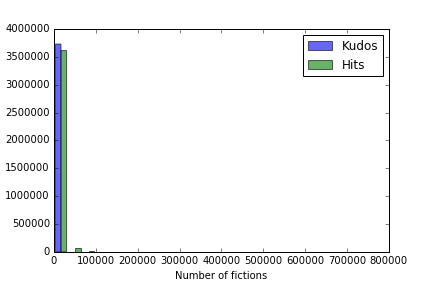
\includegraphics[width=0.6\textwidth]{/long_tail.png}
\caption{Distribution of Kudos and Hits}
\label{fig:long_tail}
\end{center}
\end{figure}


\begin{figure*}[t!]
    \centering
    \begin{subfigure}[t]{0.7\textwidth}
        \centering
        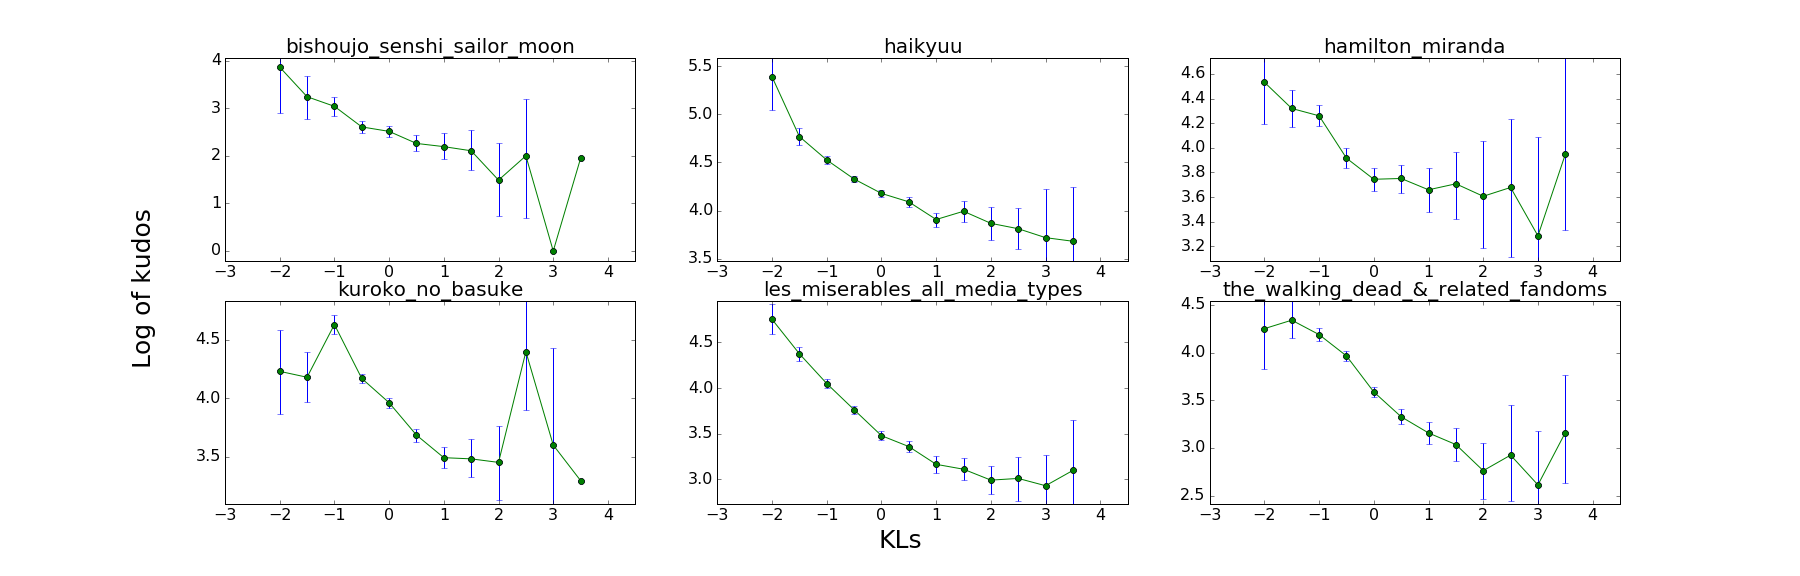
\includegraphics[height=7in]{/kl_kudos.png}
        \caption{Kudos}
    \end{subfigure}%
    ~ 
    \begin{subfigure}[t]{0.3\textwidth}
        \centering
        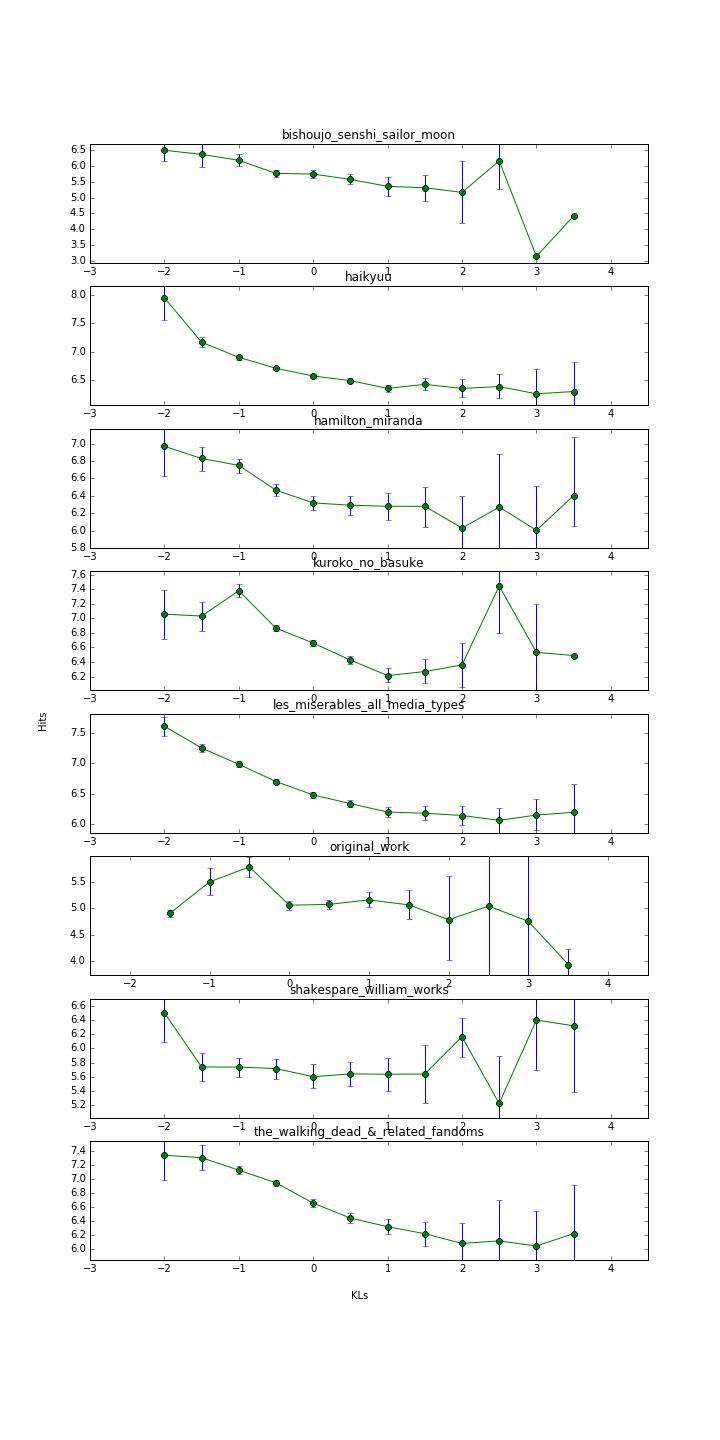
\includegraphics[height=7in]{/kl_hits.png}
        \caption{Hits}
    \end{subfigure}
    \caption{Relation between fictions' KL divergence to standard work and their Kudos or Hits in 8 fandoms. The KL divergence is turned into z-score; both Kudos and Hits are log-transformed. }
    \label{fig:kl_fields}
\end{figure*}

%}}}






\section{Results} %{{{
\label{sec:results}

%}}}

\section{Methods} %{{{
\label{sec:methods}

%}}}

\printbibliography
    
\end{document} %}}}
